\documentclass{ctexart}
\CTEXsetup[format={\Large\bfseries}]{section}            % 让section靠左对齐
\usepackage{graphicx} % Required for inserting images
\usepackage{enumerate} % 下面1,2,3小点


% 设置 subsection 的间距
\usepackage{titlesec}
\titlespacing{\section}{0pt}{0.75\baselineskip}{0.75\baselineskip}
\titlespacing{\subsection}{0pt}{0.5\baselineskip}{0.5\baselineskip}

\usepackage{geometry} % 调整页边距和纸张大小
\geometry{a4paper,scale=0.7} 

\title{\vspace{-2cm}\textbf{程序设计基础课程设计报告} \\ \fontsize{12}{14}{---高精度计算}}

\author{高宇轩 23009200132}
\date{\today}

\begin{document}
    
    \maketitle
    
    \section{原始题目及要求}
    用整型数组表示10进制大整数(超过$2^{32}$的整数),数组的每个元素存储大整数的一位数字,实现大整数的加减法。
    
    \section{题目分析}
        
    \subsection{题目功能}
    对于超过$2^{32}$的整数,超出了int能够存储的最大值,此时需要用整型数组来表示十进制的整数,我们可以用模拟竖式加减法的方式对数组进行运算。
    \subsection{题目知识点}
    数组、流程控制、函数等
    
    \section{题目总体方案设计}
    
    \subsection{程序包含的模块结构图}
    \begin{figure}[h] % 'h' 表示将图片放置在当前位置
        \centering
        
\includegraphics[width=0.8\textwidth]{parts.png}
        \caption{程序的模块结构图}

    \end{figure}
    \subsection{输入输出数据说明}
    输入数据:两个任意大小,可正可负可为零的整数
    
    输出数据:分别输出这两个整数的和与差
    \subsection{数据结构说明}
    将大整数存入bigInt类中,用一个bool变量维护整数的正负,用一个vector<int>存储整数的每一个数位
    
    \section{各功能模块的设计说明}
    \subsection{整数输入}
    先将输入的大整数存入字符串中,根据字符串首位是否为'-'判断整数的正负,然后将整数按位依次存入vector<int>中
    
    \subsection{整数相加}
    先判断两个数的符号,如果都为正或都为负,那么直接将两个数的绝对值相加,并且答案的符号与两个数相同;如果两个数为一正一负,那么用第一个数减去负的第二个数,此时问题转化为两个正数或者两个负数相减。
    
    在将两个数的绝对值相加时,从低位至高位模拟两个数的竖式加法,如果同位的两个数相加大于十,那么答案的这一位为两个数相加减十,同时向下一位的加法进位,如果出现两个数长度不同,则用零补足,直到全部加完。
    
    \subsection{整数相减}
    同样先判断两个数的符号,如果都为正或都为负,那么先判断结果的正负,然后用大的绝对值减去小的绝对值;如果两个数为一正一负,那么用第一个数加上负的第二个数,此时问题转化为两个正数或者两个负数相加。
    
    在用大的绝对值减去小的绝对值时,从低位至高位模拟两个数的竖式减法,如果相减小于零,从前一位借位,如果出现两个数长度不同,则用零补足,直到全部减完。
    
    \subsection{整数输出}
    重载<<运算符,先将bigInt转化为字符串,然后输出字符串。
    
    将bigInt转化为字符串时,先将数组中的数从高位至低位放入字符串中,同时用一个bool值判断是否为前导零。将数写入字符串后,如果字符串为空,把字符串赋值为零字符,如果不为空且有负号,在字符串前加上负号,最后输出这个字符串。
    
    \section{程序的集成测试}
    
    \begin{figure}[h] % 'h' 表示将图片放置在当前位置
    \centering
    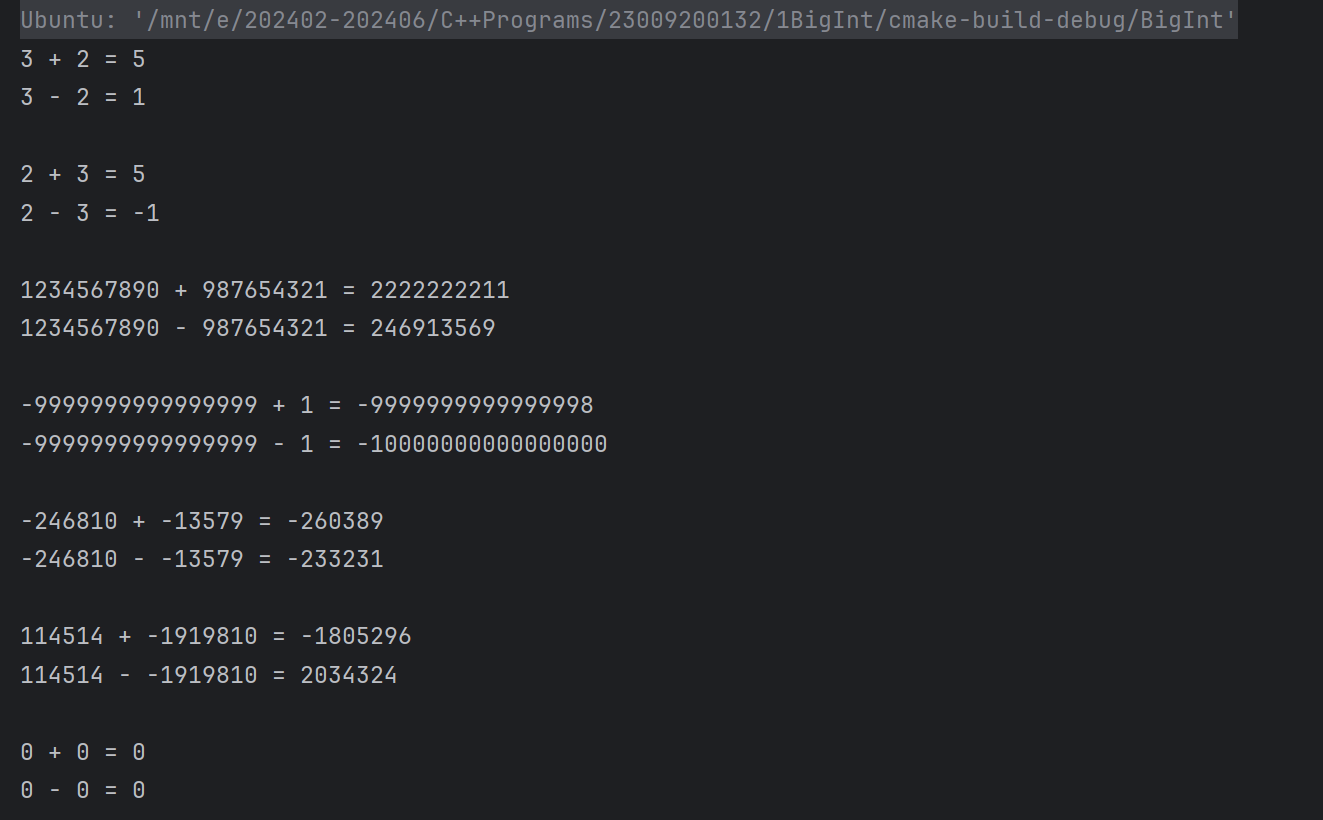
\includegraphics[width=1\textwidth]{tests.png}
    \caption{程序的集成测试}
        
    \end{figure}
    
    \section{总结}
    在集成测试中,我们分别测试了两个正数,一个正数与一个负数,一个负数与一个正数,两个负数,以及两个都为零的特殊情况,可以看出程序的运行结果都是符合我们预期的,实现了题目的要求。
    
    在今后的改进中,我们还可以用模拟整数乘法的方式,尝试编写两个大整数的乘法,进一步扩展我们的bigInt类。

    
\end{document}
